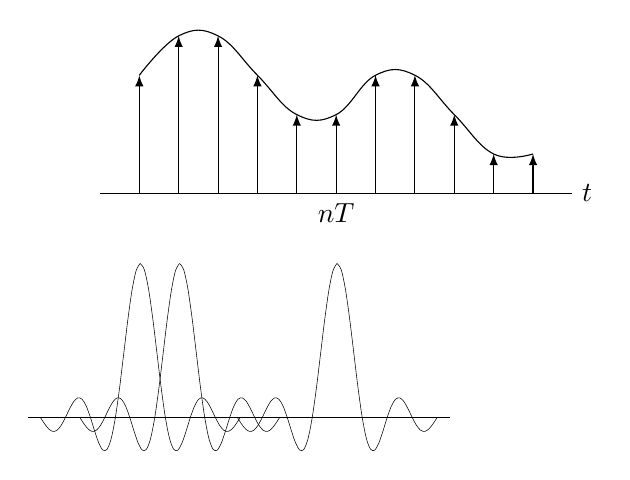
\begin{tikzpicture}[scale=0.5]
	


\draw  plot[smooth, tension=.7] coordinates {(-5,0) (-4,1) (-3,1) (-2,0) (-1,-1) (0,-1) (1,0) (2,0) (3,-1) (4,-2) (5,-2)};
\foreach \x/\y in { -5/0,  -4/1,  -3/1,  -2/0,  -1/-1,  0/-1,  1/0,  2/0,  3/-1,  4/-2,  5/-2}
{
	\draw[-latex] (\x, -3) -- (\x, \y);
}
\draw (-6, -3) -- ++(12, 0) node[anchor=west] {$t$};
\node at (0, -3) [anchor=north] {$nT$};
\begin{scope}[xshift=-3.4cm, yshift=-10cm,]
\begin{axis}
[
	axis lines=none,
]
	\addplot[domain=-4*pi:-pi/100, smooth] {0.2*sin(deg(x))/deg(x)};
	\addplot[domain=-pi/100:4*pi, smooth] {0.2*sin(deg(x))/deg(x)};
	\addplot[domain=-pi/100:4*pi] plot coordinates {(-4.5*pi, 0) (4.5*pi, 0)};
\end{axis}
\end{scope}
\pause
\begin{scope}[xshift=-8.4cm, yshift=-10cm,]
\begin{axis}
[
	axis lines=none,
]
	\addplot[domain=-4*pi:-pi/100, smooth] {0.2*sin(deg(x))/deg(x)};
	\addplot[domain=-pi/100:4*pi, smooth] {0.2*sin(deg(x))/deg(x)};
	\addplot[domain=-pi/100:4*pi] plot coordinates {(-4.5*pi, 0) (4.5*pi, 0)};
\end{axis}
\end{scope}

\pause
\begin{scope}[xshift=-7.4cm, yshift=-10cm,]
\begin{axis}
[
	axis lines=none,
]
	\addplot[domain=-4*pi:-pi/100, smooth] {0.2*sin(deg(x))/deg(x)};
	\addplot[domain=-pi/100:4*pi, smooth] {0.2*sin(deg(x))/deg(x)};
	\addplot[domain=-pi/100:4*pi] plot coordinates {(-4.5*pi, 0) (4.5*pi, 0)};
\end{axis}
\end{scope}

\end{tikzpicture} 